\documentclass[../main/main.tex]{subfiles}

\begin{document}

\section{Python Testing} 

\subsection{Setting up in Pycharm}

A new Python 3.4 project was created in Pycharm. This turned out to be
very easy, so it is not necessary to revise the steps that I went
through. 

Afterwards, I created a module in the root directory called
\lstinline|bruch|. In this module I wrote the class \lstinline|Bruch|
by overriding all the necessary magic functions,
e.g. \lstinline|__add__()|, \lstinline|__isub__()|, that were used in
the given tests.

The tests were included in a separate directory called
\lstinline|test|. Afterwards, I created a run configuration that
executed all tests in the previously mentioned \lstinline|test|
directory. The configuration can be seen in Figure \ref{fig:edit}.

\begin{figure}[H]
  \centering
  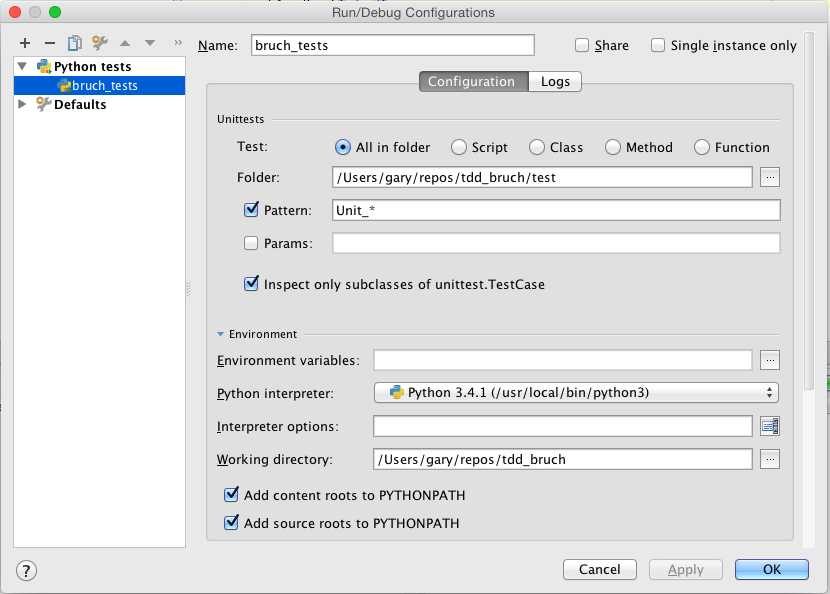
\includegraphics[width=0.7\linewidth]{../figures/edit_config.png}
  \caption{Edit configuration for tests}
  \label{fig:edit}
\end{figure}

A simple hit on the run button will execute all the tests
appropriately.

\subsection{Coverage Report (HTML) in Pycharm}

By selecting the \textit{Run with Coverage} option, one
can also generate a coverage report, which can take a while. 

An HTML report can be generated by first running the \textit{Run with
  Coverage} option, and subsequently selecting \textit{Tools/Generate
  Coverage Report}.

The report of this exercise, which are generated in HTML files, can be
found in the \textit{report/} directory, but can also be seen in
Figure \ref{fig:coverage}. 

\begin{figure}[H]
  \centering
  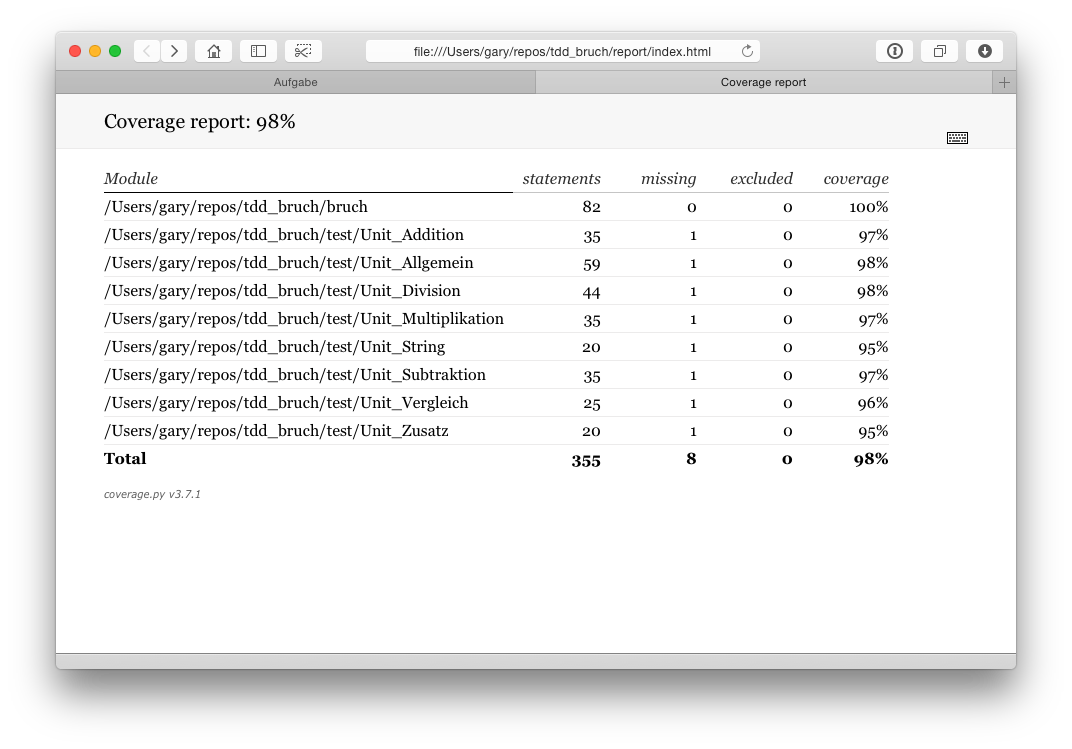
\includegraphics[width=\linewidth]{../figures/coverage_report.png}
  \caption{Coverage report}
  \label{fig:coverage}
\end{figure}

The fraction class was written such that it passed all test cases,
which was successful as we can see in Figure \ref{fig:unit}, which is
a screenshot from the test report generated by Pycharm. The report can be generated by clicking on the ``Export'' button in, as seen in \ref{fig:export}.

\begin{figure}[H]
  \centering
  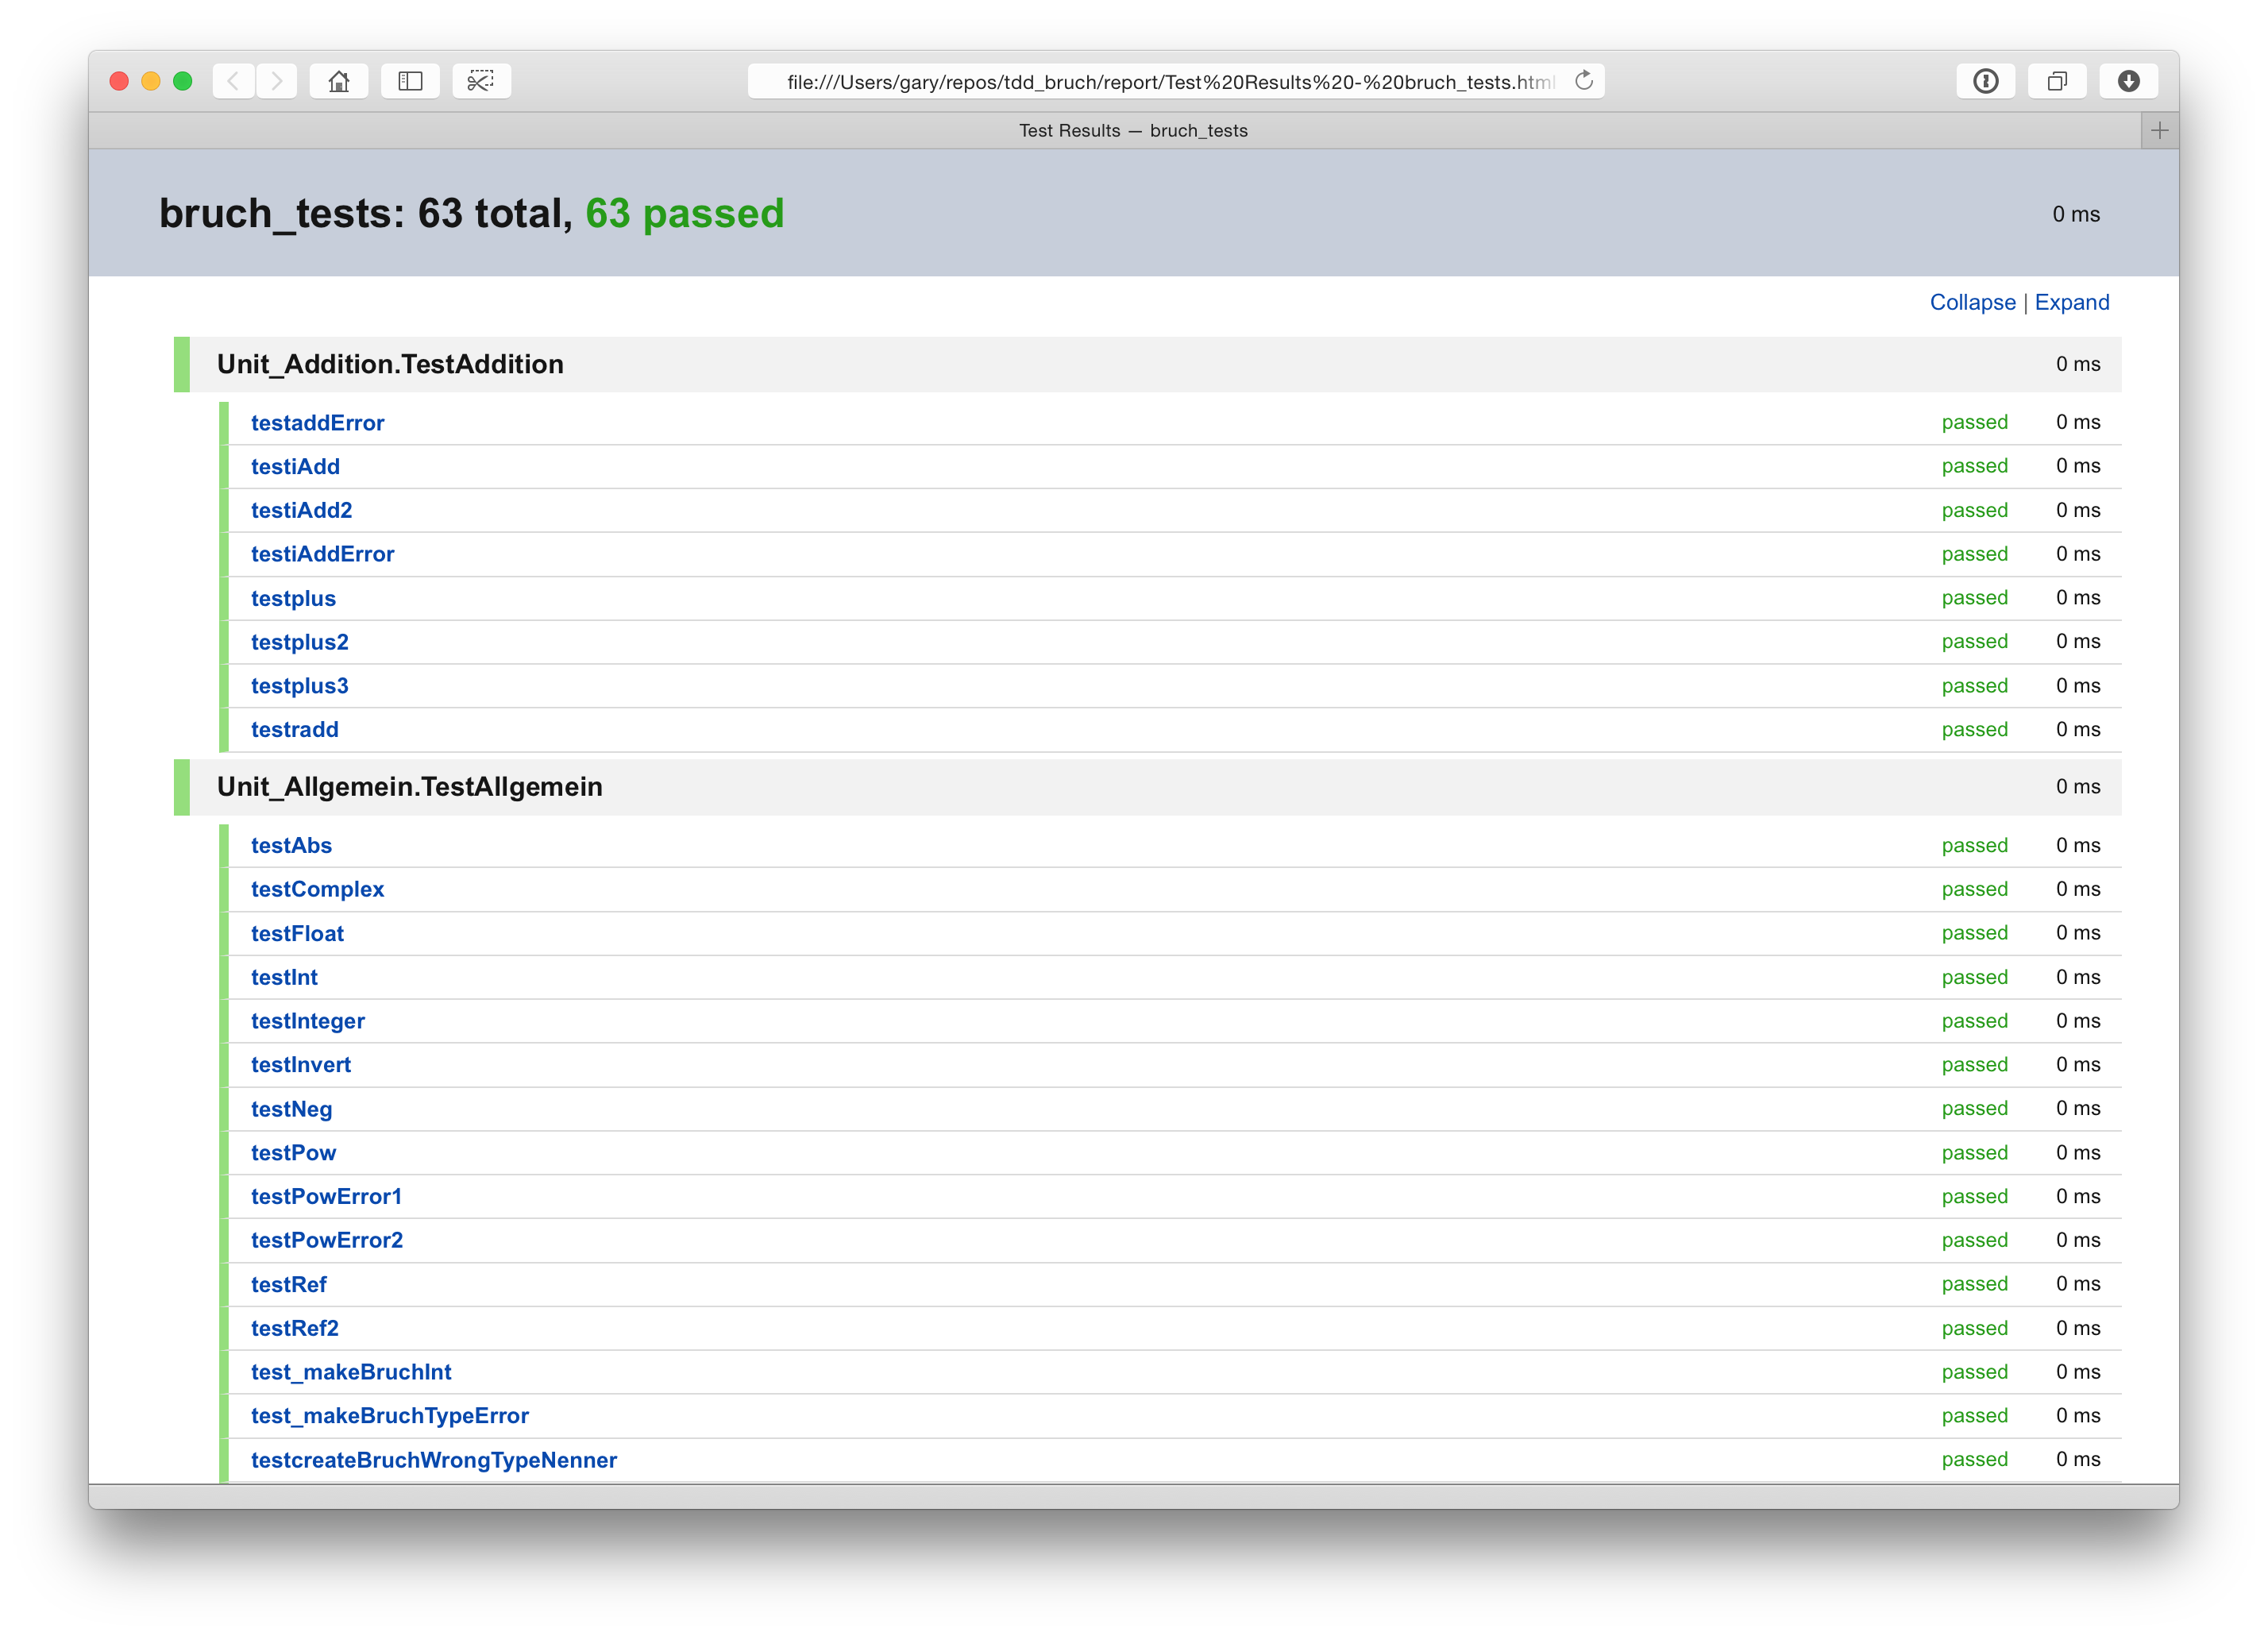
\includegraphics[width=0.7\linewidth]{../figures/unit_testing.png}
  \caption{Unit testing.}
  \label{fig:unit}
\end{figure}

\begin{figure}[H]
  \centering
  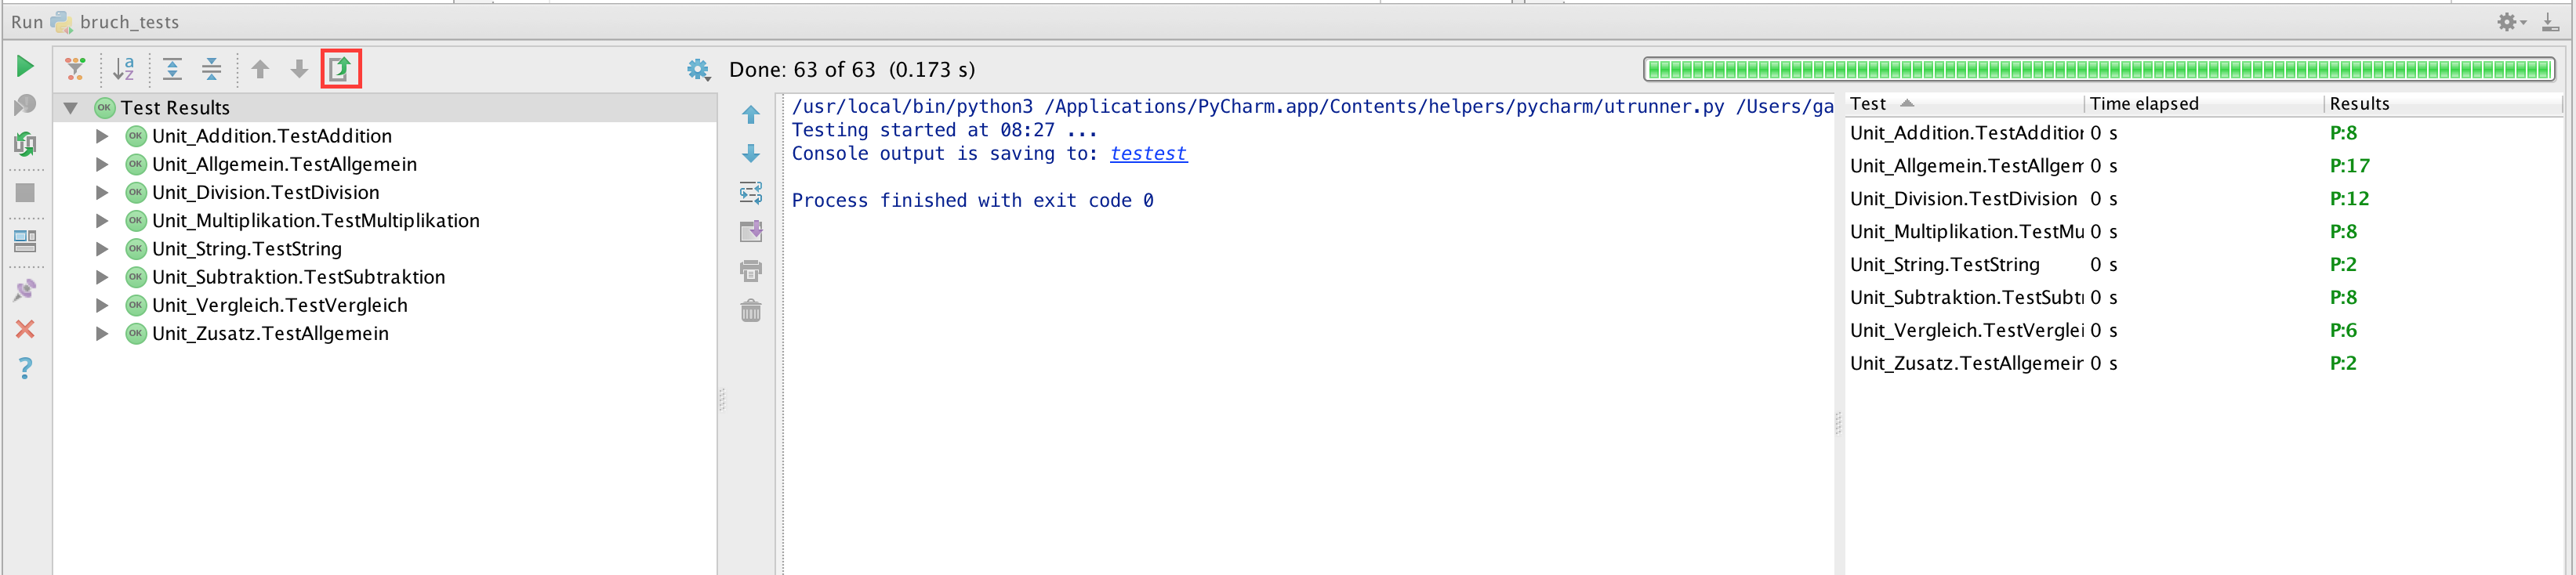
\includegraphics[width=0.8\linewidth]{../figures/export.png}
  \caption{Exporting the unit tests.}
  \label{fig:export}
\end{figure}

\subsection{Creating Test-Suites}

A test suite defines a set of test cases that should be ran together.
Fortunately, \lstinline|unittest| also provides the \lstinline|TestSuite| class
that can be used to add each test case that should be inside the suite. 

The test suite must be started with the \lstinline|unittest.TextTestRunner()|. 

\begin{lstlisting}
import unittest

from tests.models.test_follow import FollowTest


def suite():
    test_suite = unittest.TestSuite()
    test_suite.addTest(unittest.makeSuite(FollowTest))
    return test_suite

if __name__ == '__main__':
    unittest.TextTestRunner().run(suite())
\end{lstlisting}

\subsection{Flask-Testing}

Using the Flask-Testing package, testing is substantially simpler. However, we
still want to define a base test case such as the following class:

\begin{lstlisting}
from app import create_app
from app.config import TestConfiguration
from flask.ext.testing import TestCase

from app.extensions import db

class BaseTestCase(TestCase):
    """
    Classes that inherit this class are able to test with the config.TestConfiguration setup that is provided in
    config.py.
    """

    def create_app(self):
        return create_app(TestConfiguration)

    def setUp(self):
        db.create_all()

    def tearDown(self):
        db.session.remove()
        db.drop_all()
\end{lstlisting}

For instance, other classes can derive from the aforementioned class and get
more features. 

\begin{lstlisting}
from app.models import User
from flask import url_for
from flask.ext.login import current_user
from tests.test_base import BaseTestCase


class UserViewsTests(BaseTestCase):
    def test_users_can_login(self):
        User.create(username='joe', password='12345')
        response = self.client.post(url_for('user.login'), data={'name': 'joe', 'password': '12345'})
        self.assert_redirects(response, url_for('user.index'))

    def test_users_can_logout(self):
        User.create(username='joe', password='12345')

        with self.client:
            self.client.post(url_for('user.login'), data={'name': 'joe', 'password': '12345'})
            self.client.get(url_for("user.logout"))
            self.assertTrue(current_user.is_anonymous())
\end{lstlisting}

\subsection{Selenium Testing}

Selenium testing is easy as it seems. We have to use the
\lstinline|LiveServerTestCase| as it can spawn a new LiveServer, which is very
helpful for our Selenium tests. 

In \lstinline|test_login| we can see some of the available Selenium commands.
More of them can be found in the official Selenium webdriver documentation. 

\begin{lstlisting}
import os
from app import create_app
from app.config import TestConfiguration
from app.extensions import db
from app.models import User
from flask.ext.testing import LiveServerTestCase
from selenium import webdriver


class LiveServerTestBase(LiveServerTestCase):
    def create_app(self):
        self.app = create_app(TestConfiguration)
        return self.app

    def init_data(self):
        db.create_all()
        User.create(username='gary', password='password')

    def setUp(self):
        self.init_data()
        self.browser = webdriver.Chrome() # or Firefox

    def tearDown(self):
        db.drop_all()
        os.unlink(self.app.config['DATABASE'])
        self.browser.quit()

    def test_visit(self):
        self.browser.get(self.get_server_url() + '/user/login')

    def test_login(self):
        self.browser.get(self.get_server_url() + '/user/login')
        name_form = self.browser.find_element_by_id('name')
        pwd_form = self.browser.find_element_by_id('password')
        submit_form = self.browser.find_element_by_id('submit')
        name_form.send_keys('gary')
        pwd_form.send_keys('password')
        submit_form.click()

        self.assertIn('Login successful', self.browser.page_source)

\end{lstlisting}

\end{document}
